\chapter{Automatic generator}
The automatic generator of Gr\"obner basis solvers is used to easily solve problems leading to systems of polynomial equations. These systems usually arise when solving minimal problems \cite{MinimalProblems} in computer vision. Typically, these systems are not trivial so special solvers have to be designed for concrete problems to achieve efficient and numerically stable solvers. But solvers generated for concrete problems can not be easily applied for similar or new problems and therefore the automatic generator was proposed in \cite{AutoGen}. Solvers generated by the automatic generator can be easily used to solve complex problems even by non-experts users.

The input of the automatic generator is a system of polynomial equations with a finite number of solutions and the output is a MATLAB or a Maple code that computes solutions of the given system for arbitary coefficients. One of the goals of this thesis is to improve previous implementation \cite{AutoGen} of the automatic generator to construct more efficient and numerically stable solvers.

The newest version of the automatic genenerator implemented in MATLAB can be downloaded from \cite{AutomaticGenerator}.

\section{Description of the automatic generator}
In this section we would like to briefly describe the procedure for generating solvers. The procedure is based on computation of the action matrix from which solutions can be obtained. The automatic generator consists of several independent modules, see Figure \ref{autogen:blockDiagram}. Since all these modules are independent, they can be easily improved or replaced by more efficient implementations. Next we describe each of these modules, full description can be found in \cite{AutoGen, KukelovaAlgMethods}.

\begin{figure}[ht]
  \centering
  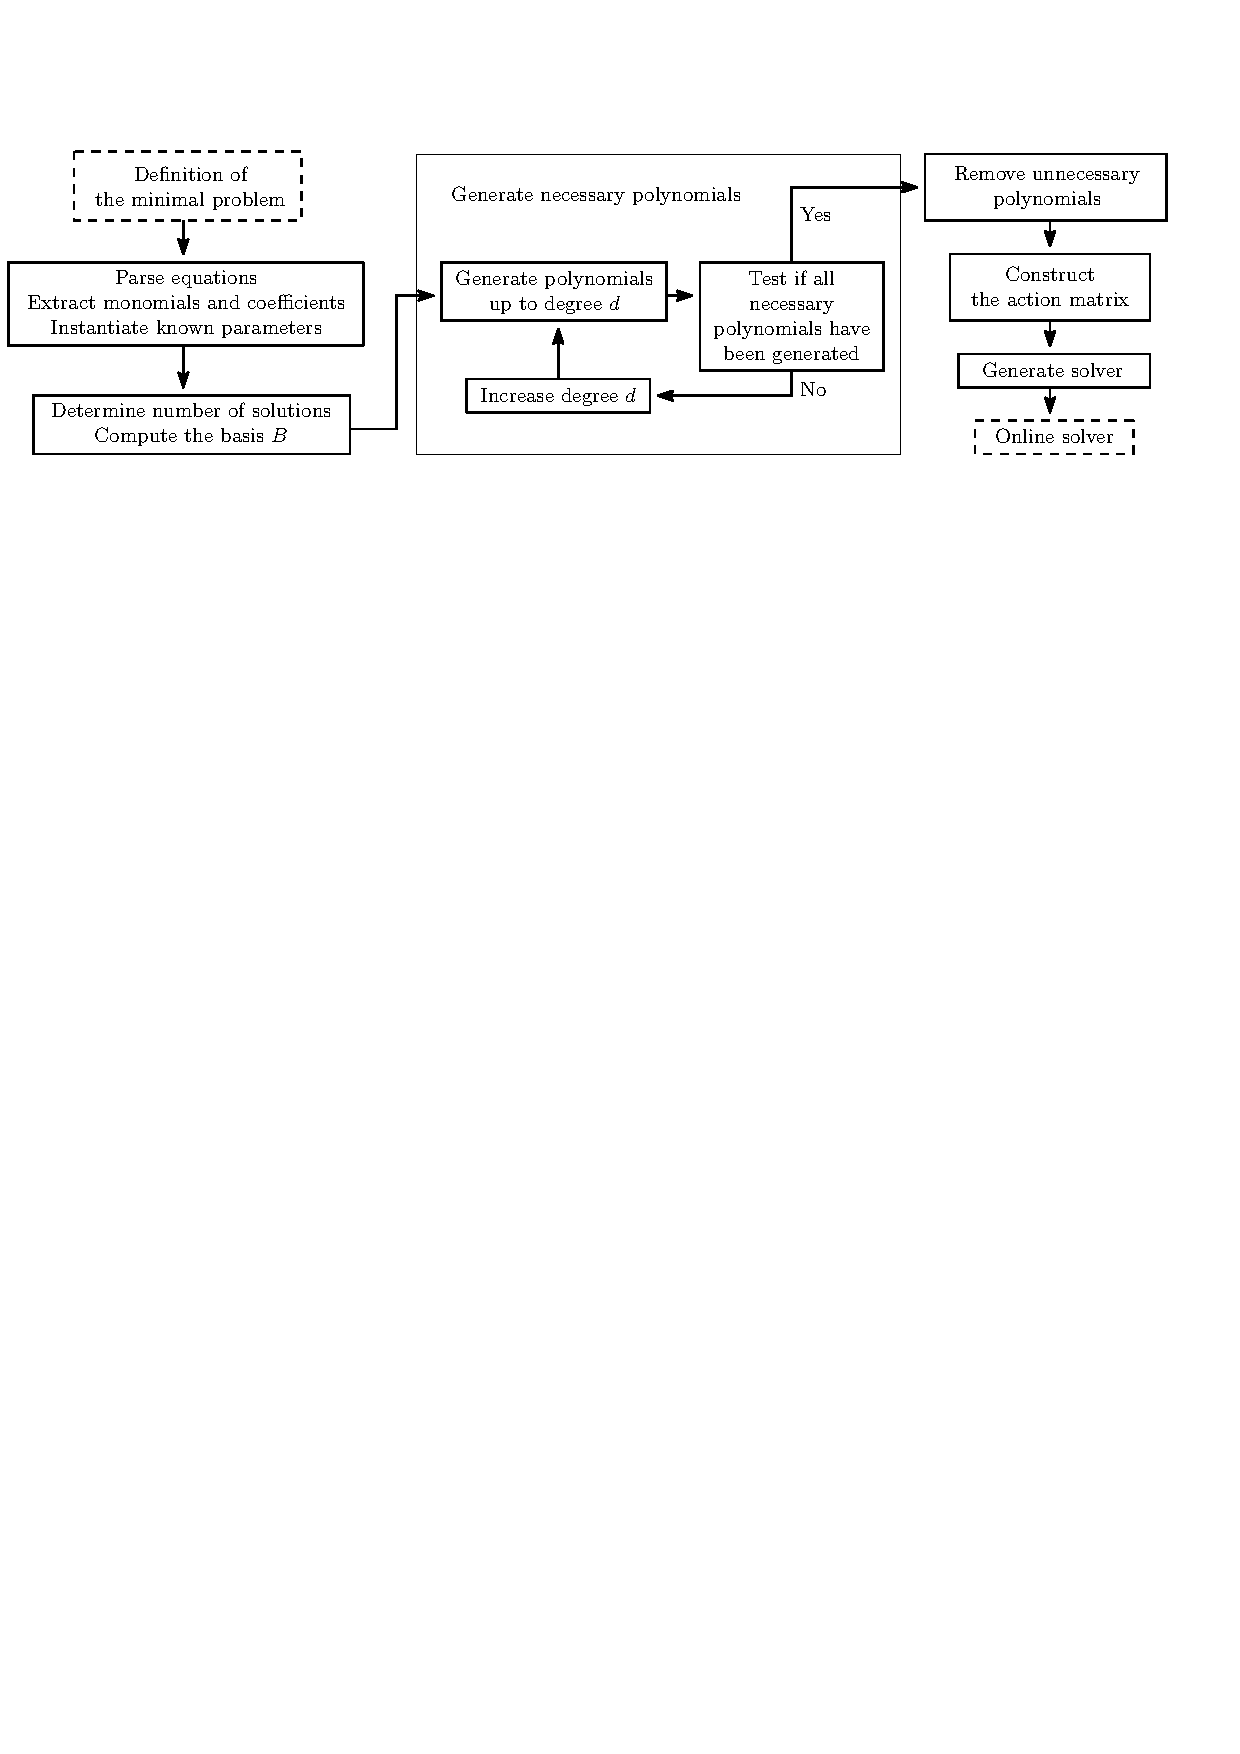
\includegraphics[width=0.95\textwidth]{AutomaticGenerator.pdf}
  \caption{Block diagram of the automatic generator}
  \label{autogen:blockDiagram}
\end{figure}

\subsection{Definition of the minimal problem}
\label{subsec:MinimalProblemDefinition}
Definitions of minimal problems are written in separate functions that are stored in the folder \texttt{minimalProblems}. Each of the definitions has to contain few necessary information about the minimal problem. First of all, the system of polynomial equations with symbolic variables and parameters has to be provided. Next we have to specify the list of unknown variables and known parameters. Optionally if we know the monomial basis $B$ of the polynomial system in advance we can specify it to save some computation time. The monomial basis $B$ is a set $\left\{m\ |\ \overline{m}^G = m\right\}$ where $m$ is a monomial and $G$ is the Gr\"obner basis of the given polynomial system. At last we have to set some settings for the automatic generator. We recommend to obtain the default settings by calling the function \textit{gbs\_InitConfig()} and only overwrite the settings we want to change. In the folder \texttt{minimalProblem} there are some examples which are self explanatory and can be used as templates to create new minimal problem definitions.

\subsection{Equations parser, Instantiating}
In the next step we have to parse the given equations, that means we extract used monomials and parameters and obtain total degrees of the polynomials. Then we instantiate each known parameter with a random number from $\mathbb{Z}_p$. We assign unique identifier to each used parameter. The reason is that we need to track the parameters through the process of adding polynomials in order to be able to restore the process in the solver generation module.

\subsection{Monomial basis $B$ computation}
We need to know the monomials basis $B$ to recognize when we have generated all polynomials that are necessary to build the action matrix. If the basis $B$ was not provided within the definition of the minimal problem we have to compute it by ourselves. Because in MATLAB there is no function or simple script to compute the basis we have to do it by calling an external software.

The most easy solution to implement was to use the Maple toolbox for MATLAB. This enables us to call Maple functions from the MATLAB environment directly. To use this option we have to set \texttt{cfg.GBSolver = @gbs\_findAlgB\_maple} in the settings of the automatic generator. Unfortunately it shows up that the symbolic toolbox provided by Maple in not compatible with the MATLAB symbolic toolbox in versions newer than R2008 so we do not recommend to use this option nowadays, but the option is still available to use on older computers.

The second implemented option is to use the algebraic geometry software Macaulay2 \cite{M2}. In the folder \texttt{gbsMacaulay} there is a template \texttt{code\_template.m2} into which we simply write the given polynomial system. This updated file is saved as \texttt{code.m2} which is executed by Macaulay2 and the results are parsed back in MATLAB. To set up this option we need to install the software Macaulay2 and set \texttt{cfg.GBSolver = @gbs\_findAlgB\_macaulay} in the automatic generator settings. A problem could be that the Macaulay2 is not easy to set up under the Windows OS. Therefore the installation file of Macaulay2 is provided within the automatic generator. The only thing that has to be done is to edit the file \texttt{calc.bat} in the folder \texttt{gbsMacaulay} and follow the instructions in the file.

Because of the modularity of the generator this part can be replaced by another function computing the monomial basis $B$.

The last option is to compute the basis $B$ in advance and set it into the definition of the minimal problem.

In the end we have check the number of solutions of the given polynomial system. If there is a finite number of solutions we can continue with the computation.

\subsection{Polynomial generator}
To be able to build the action matrix we have to generate enough polynomials such that after their reduction we get polynomials $q_i$ which have leading monomials from the set $\left(x_k \cdot B\right)\backslash B$ where $x_k$ is a variable and all remaining monomials of $q_i$ are from the set $B$. That is the reason we had to compute the basis $B$ in the previous step.

In this part of the automatic generator we represent polynomials as row vectors so systems of polynomials can be represented by matrices. This representation enables us to easily multiplicate polynomials with monomials only by shifting the coefficients in the vectors or to reduce the whole polynomial systems by performing the Gauss-Jordan eliminations on the corresponding matrices.

Let $f_i \in F$ where $F$ is a set of polynomials from the input. Let $maxdeg$ is a maximal total degree of all polynomials $f_i$. At the beginning we put into the matrix $M$ all polynomials $\left\{m\times f_i\ |\ f_i \in F;\ \deg(m\times f_i) = \deg(f_i),\dots, maxdeg\right\}$, where $m$ is a monomial. Now we perform the Gauss-Jordan elimination on the matrix $M$ and the result save as matrix $\tilde{M}$. Then we check if there exists a variable $x_k$ for which all required polynomials $q_i$ are present in $\tilde{M}$. If we find such a variable we can continue with the construction of the action matrix for the found variable. If not we have to add more polynomials to the matrix $M$. We increment $maxdeg$ by one and add all polynomials $\left\{m\times f_i\ |\ f_i \in F;\ \deg(m\times f_i) = maxdeg\right\}$ to the matrix $M$. Then we continue with the elimination and with the checking the action matrix requirements as written above. We repeat these steps until all required polynomials $q_i$ are generated so the action matrix can be built. The pseudocode of this process is shown in Algorithm \ref{alg:oneElGen}. The function \textit{Check Action Matrix Conditions} from this code checks if all polynomials $q_i$ are generated in $\tilde{M}$ for at least one variable from the given list of variables. If such a variable is found the function returns it otherwise it returns an empty set.

\begin{algorithm}[ht]
  \begin{algorithmic}[1]
    \Require
      \Statex $F$ a set of polynomials
      \Statex $variables$ a list of variables
      \Statex $algB$ a monomial basis $B$
    \Ensure
      \Statex $\tilde{M}$ a matrix representing a set of polynomials
      \Statex $var$ a variable
      \Statex

    \State $maxdeg \gets \max\{\deg(f_i)\ |\ f_i \in F\}$
    \State $M \gets \left\{m f_i\ |\ f_i \in F;\ \deg(m f_i)\ =\ \deg(f_i),\dots,maxdeg;\ m \textrm{ is a monomial} \right\}$
    \State $\tilde{M} \gets$ Reduction to a Row Echelon Form of $M$
    \State $var \gets Check\ Action\ Matrix\ Conditions(\tilde{M}, variables, algB)$
    \While{$var = \emptyset$}
      \State $maxdeg \gets maxdeg + 1$
      \State $M \gets M \cup \left\{m f_i\ |\ f_i \in F;\ \deg(m f_i)\ = \ maxdeg;\ m \textrm{ is a monomial}\right\}$
      \State $\tilde{M} \gets$ Reduction to a Row Echelon Form of $M$
      \State $var \gets Check\ Action\ Matrix\ Conditions(\tilde{M}, variables, algB)$
    \EndWhile
    \State \Return $(\tilde{M}, var)$
  \end{algorithmic}
  \caption{Polynomial generator -- One elimination solver}
  \label{alg:oneElGen}
\end{algorithm}



In this whole process we need to keep track how the matrix $M$ was built. Recall that each coefficient of the polynomials $f_i$ has unique identifier assigned in the equations parser. Because the whole matrix $M$ contains only the polynomials $f_i$ or their multiples with monomials therefore in the matrix $M$ appear only the coefficients from the polynomials $f_i$. We just have to keep the positions of the coefficients. This is done by matrix $M_c$. The matrix $M_c$ is built in the same time as the matrix $M$ by this way: if we put a coefficient into the matrix $M$ we also put the corresponding indentifier to the matrix $M_c$ at the same possition. The matrix $M_c$ enables us to recover the process of polynomials generation in the code generator module.

\subsection{Removing unnecessary polynomials and monomials}
Since in the previous step the polynomials were generated systematically there may appear some polynomials which are not necessary for the constructing of the action matrix. The goal of this part of the automatic generator is to remove as many as possible not necessary polynomials.

We can remove a polynomial $r$ from the matrix $M$ if the corresponding eliminated matrix $\tilde{M}$ still contains all required polynomials $q_i$. In this way we try to remove all polynomials from $M$.

Because the success of removing a polynomial depends on the previous removals, the number of removed polynomials depends on the ordering in which the polynomials are removed. In the automatic generator we start removing polynomials from the one with the largest leading monomial to the polynomial with the smallest leading monomial in order by monomial ordering used. Because it is very inefficient to remove polynomials one by one and perform each time an expensive Gauss-Jordan elimination, we can enhance the procedure by trying to remove more polynomials at the time. In the automatic generator there is used this heuristic: if we have successfully removed $k$ polynomials, we try to remove $2\cdot k$ polynomials in the next step. If the removal of $k$ polynomials have failed we try to remove $\frac{1}{4}k$ polynomials in the next step. The pseudocode of this removing process is shown as Algorithm \ref{alg:removeUn}.

\begin{algorithm}[!ht]
  \begin{algorithmic}[1]
    \Require
      \Statex $M$ a matrix representing a set of polynomials
      \Statex $variable$ a variable
      \Statex $algB$ a monomial basis $B$
    \Ensure
      \Statex $M$ a matrix representing a set of polynomials
      \Statex

      \State $rows \gets$ number of rows of $M$
      \State $step \gets \max\{\lfloor rows/32\rfloor, 1\}$ 
      \State $up \gets 1$
      \State $filter \gets \{1,2,\dots,rows\}$
      \While{$up \leq rows$}
        \State $down \gets up + step - 1$
	\If{$down > rows$}
          \State $down \gets rows$
	  \State $step \gets down - up + 1$
	\EndIf
	\State $filter_{Old} \gets filter$
	\State $filter \gets filter \backslash \{up, up+1, \dots, down\}$
	\State $\tilde{M} \gets$ Reduction to a Row Echelon Form of $M$ only with rows specified by $filter$
        \State $v \gets$ \textit{CheckActionMatrixConditions}$(\tilde{M}, variable, algB)$
	\If{$v = variable$}
          \State $up \gets down + 1$
	  \State $step \gets 2 step$
	\Else
	  \If{$step = 1$}
	    \State $up \gets up + 1$
	  \Else
            \State $step \gets \max\{\lfloor step/4\rfloor, 1\}$
	  \EndIf
	  \State $filter \gets filter_{Old}$
	\EndIf
      \EndWhile

      \State \Return $M$ only with rows specified by $filter$
  \end{algorithmic}
  \caption{Remove unnecessary polynomials}
  \label{alg:removeUn}
\end{algorithm}



Moreover we can reduce the size of the matrix $M$ by removing unnecessary monomials. A monomial is unnecessary when its removal does not affect the building of the action matrix. We have to keep all monomials such that they are leading monomials of polynominals in the corresponding matrix $\tilde{M}$ and all monomials that are present in the basis $B$. All other monomials can be removed. If we remove all such unnecessary monomials then the matrix $M$ will have dimensions $n \times (n + N)$ where $n$ is the number of the polynomials in the matrix $M$ and $N$ is the number of solutions of the given system.

\subsection{Construction of the action matrix}
This part of the automatic generator starts with the eliminated matrix $\tilde{M}$ of polynomials and variable $x_k$ for which all required polynomials $q_i$ are present in the $\tilde{M}$.

Let us describe the construction of the action matrix in an informal and practical way rather than by using the theory. If the theory is needed it can be found in \cite{KukelovaAlgMethods}. The action matrix $M_{x_k}$ corresponding to the variable $x_k$ is a square matrix of dimensions $N \times N$ where $N$ is the number of elements of the monomial basis $B$. Each row and column corresponds to a monomial $b_i \in B$. Let the monomials $b_i$ are sorted such that if $b_l \prec b_k$ then $k < l$ where $\prec$ is a monomial ordering used. To the $i$-th row we put coefficients of the polynomial $m_i\ =\ \overline{(x_k \times b_i)}^F$ where $F$ are polynomials corresponding to $\tilde{M}$. Because $\tilde{M}$ is in a row echelon form there are two possibilities how the $i$-th row can be constructed:
\begin{enumerate}
  \item $x_k \times b_i\ =\ b_j$ for some $b_j \in B$\\
        That means that $x_k \times b_i$ is irreducible by $F$ and $m_i$ is a monomial in $B$. In this case we set $(i, j)\ =\ 1$ and $(i, k)\ =\ 0$ where $k\ \neq\ j$.
  \item $x_k \times b_i\ \neq\ b_j$ for all $b_j \in B$\\
	  In this case there is $f$ such that $\LM(m_i)\ =\ \LM(f)$ where $f \in F$ so $m_i\ =\ x_k\times b_i - f$. Since all monomials of $f$ except $\LM(f)$ are from $B$, all monomials of $m_i$ are also from $B$. On the $(i, j)$ position of the matrix $M_{x_k}$ we put coefficient of $m_i$ at the monomial $b_j$.
\end{enumerate}

Now the solutions of the given system can be easily found by computing right eigenvectors of the action matrix $M_{x_k}$.

\subsection{Solver generator}
The last task of the automatic generator is to create a solver which will solve the given polynomial system for an arbitrary set of parameters. The current version of the automatic generator can generate solvers for MATLAB and Maple, but new code generators can be easily added. Which solvers will be generated can be set in the minimal problem definition by setting \texttt{cfg.exportCode}, e.g. to create both MATLAB and Maple solvers we set \texttt{cfg.exportCode = \{'matlab' 'maple'\}}.

To create the solver we have to restore the process of creation of the matrix $M$. This process is saved as the matrix $M_c$ which contains unique identifiers on the positions where the given parameters have to be put. So the matrix $M$ can be built for each given set of parameters. Then the Gauss-Jordan elimination is called on $M$ so we get the matrix $\tilde{M}$. Now the action matrix is built in the same way as above and the solutions are extracted from it. To sum up the final solver just creates the matrix $M$ by putting parameters to the correct places. After Gauss-Jordan elimination the action matrix is built by copying some parts of rows of $\tilde{M}$ and then the solutions are extracted by using the eigenvectors of the action matrix.

\subsection{Usage}
The automatic generator is designed to be able to be used even by non-expert users and to be easily expanded or improved.

At first the script \texttt{setpaths.m} from the root directory of the automatic generator should be executed. This will add all required paths to the MATLAB environment.

Next we have to set up the definition of the minimal problem we want to solve. How the definition have to be specified is written in the section \ref{subsec:MinimalProblemDefinition}. All these definitions are stored in the folder \texttt{minimalProblems}. To generate the solver we call the function \texttt{gbs\_GenerateSolver(MinimalProblem)} where \texttt{MinimalProblem} is the name of the definition of the minimal problem, i.e. the name of the function in the folder \texttt{minimalProblems}. This will generate us solvers \texttt{solver\_MinimalProblem.m} for the MATLAB solver and \texttt{solver\_MinimalProblem.txt} for the Maple solver. These solvers are stored in the folder \texttt{solvers}.

For example we want to generate solver for the 6-point focal length problem. We have defined this problem as a function \texttt{sw6pt.m} in the folder \texttt{minimalProblems}. By calling the function \texttt{gbs\_GenerateSolver('sw6pt')} we get solvers \texttt{solver\_sw6pt.m} and \texttt{solver\_sw6pt.txt} in the folder \texttt{solvers}.

\section{Improvements}

\subsection{Reimplementation}

\subsection{Multiple eliminations solver}

\subsection{Removing unnecessary polynomials}

\subsection{Matrix partitioning}

\subsection{F4 strategy}

\section{Benchmark}
